\documentclass{beamer}
\usepackage{amsmath,amsbsy,amsopn,amstext,amsfonts,amssymb}
\usepackage{isomath}
\usepackage{ulem}
%\linespread{1.6}  % double spaces lines
\usepackage{graphicx}
\usepackage{subfigure}
\usepackage{color}
\usepackage{optidef}  % define optimization problems
\usepackage{multicol}  % multiple columns
\usepackage{listings} % for python code
\usepackage{mathrsfs}

\usepackage{polynom}
\newcommand{\adj}{\mathrm{adj}}
\newcommand{\constrainedmin}[3]{
		\begin{mini*}|s|
		{#2}{#1}{}{}
		\addConstraint{#3}
		\end{mini*}
}

\newcommand{\rwbcomment}[1]{{\color{blue}RWB:#1}}
\newcommand{\defeq}{\stackrel{\triangle}{=}}
\newcommand{\abs}[1]{\left|#1\right|}
\newcommand{\norm}[1]{\left\|#1\right\|}
\newcommand{\iprod}[1]{\left<#1\right>}
\newcommand{\ellbf}{\boldsymbol{\ell}}
\newcommand{\nubf}{\boldsymbol{\nu}}
\newcommand{\mubf}{\boldsymbol{\mu}}
\newcommand{\abf}{\mathbf{a}}
\newcommand{\bbf}{\mathbf{b}}
\newcommand{\cbf}{\mathbf{c}}
\newcommand{\dbf}{\mathbf{d}}
\newcommand{\ebf}{\mathbf{e}}
\newcommand{\fbf}{\mathbf{f}}
\newcommand{\gbf}{\mathbf{g}}
\newcommand{\hbf}{\mathbf{h}}
\newcommand{\ibf}{\mathbf{i}}
\newcommand{\jbf}{\mathbf{j}}
\newcommand{\kbf}{\mathbf{k}}
\newcommand{\lbf}{\mathbf{l}}
\newcommand{\mbf}{\mathbf{m}}
\newcommand{\nbf}{\mathbf{n}}
\newcommand{\obf}{\mathbf{o}}
\newcommand{\pbf}{\mathbf{p}}
\newcommand{\qbf}{\mathbf{q}}
\newcommand{\rbf}{\mathbf{r}}
\newcommand{\sbf}{\mathbf{s}}
\newcommand{\tbf}{\mathbf{t}}
\newcommand{\ubf}{\mathbf{u}}
\newcommand{\vbf}{\mathbf{v}}
\newcommand{\wbf}{\mathbf{w}}
\newcommand{\xbf}{\mathbf{x}}
\newcommand{\ybf}{\mathbf{y}}
\newcommand{\zbf}{\mathbf{z}}
\newcommand{\Jbf}{\mathbf{J}}
\newcommand{\Acal}{\mathcal{A}}
\newcommand{\Bcal}{\mathcal{B}}
\newcommand{\Lcal}{\mathcal{L}}
\newcommand{\Ncal}{\mathcal{N}}
\newcommand{\Rcal}{\mathcal{R}}
\definecolor{darkolivegreen}{rgb}{0.33, 0.42, 0.18}

\makeatletter
\newenvironment<>{proofstart}[1][\proofname]{%
    \par
    \def\insertproofname{#1\@addpunct{.}}%
    \usebeamertemplate{proof begin}#2}
  {\usebeamertemplate{proof end}}
\newenvironment<>{proofcont}{%
  \setbeamertemplate{proof begin}{\begin{block}{}}
    \par
    \usebeamertemplate{proof begin}}
  {\usebeamertemplate{proof end}}
\newenvironment<>{proofend}{%
    \par
    \pushQED{\qed}
    \setbeamertemplate{proof begin}{\begin{block}{}}
    \usebeamertemplate{proof begin}}
  {\popQED\usebeamertemplate{proof end}}
\makeatother

\title{ECEn 671: Mathematics of Signals and Systems}
\author{Randal W. Beard}
\institute{Brigham Young University}
\date{\today}

\begin{document}

%-------------------------------
\begin{frame}
	\titlepage
\end{frame}

%%%%%%%%%%%%%%%%%%%%%%%%%%%%%%%%%%%%%%%%%%%%%%%%%%%%%%%%%%%%%%%%%
\section{Linear Operators}
\frame{\sectionpage}


%----------------------------------
\begin{frame}\frametitle{Linear Operators}
	Recall from Chapter~3 the definition of a Linear operator:  
	\begin{definition}
	Let $\mathbb{X}$ and $\mathbb{Y}$ be vector spaces, then $\mathcal{A}:\mathbb{X} \to \mathbb{Y}$ is a linear operator if
	\[ 
	\mathcal{A}[\alpha_1 x_1 + \alpha_2 x_2 ] = \alpha_1 \mathcal{A}[x_1] + \alpha_2 \mathcal{A}[x_2] 
	\]	
	$\forall x_1,x_2 \in \mathbb{X}$ and $\forall \alpha_1,\alpha_2 \in \mathbb{F}$
	\end{definition}
	
	\vfill
	See chapter 2 notes (slides 79--83) for examples of linear operators.
\end{frame}

%----------------------------------
\begin{frame}\frametitle{Norm of a Linear Operator}
	An important concept is the \underline{norm} of an operator.  There are several ways to define norms for operators.  The most important is the ``induced'' or ``subordinate'' norm.
	
	\vfill
	
	\begin{definition}
		Let $\mathcal{A}:\mathbb{X} \to \mathbb{Y}$ then
		\begin{align*}
		\norm{\mathcal{A}} &= \sup_{x \neq 0} \frac{\norm{\mathcal{A}[x]}_{\mathbb{Y}}}{\norm{x}_{\mathbb{X}}} \\
		&= \sup_{\norm{x}_{\mathbb{X}}=1} \norm{\mathcal{A}[x]}_{\mathbb{Y}} 
		\end{align*}
	\end{definition}
	
	\vfill
	
	Different norms on $\mathcal{A}$ are defined by taking different norms in $\mathbb{X}$ and $\mathbb{Y}$.
\end{frame}

%----------------------------------
\begin{frame}\frametitle{Norm of a Linear Operator, Examples}
	\begin{example}
	Let $\mathcal{A}: L_2 \to L_2$ then
	\begin{align*}
	\norm{\mathcal{A}}_2 &= \sup_{x \neq 0} \frac{\norm{\mathcal{A}[x]}_{L_2}}{\norm{x}_{L_2}} \\
	&= sup_{\norm{x}_{L_2} = 1} \norm{\mathcal{A}[x]}_{L_2} 
	\end{align*}
	\end{example}
	
	\begin{example}
		Let $\mathcal{A}: L_{\infty} \to L_{\infty}$ then
		\begin{align*}
			\norm{\mathcal{A}}_{\infty} &= \sup_{x \neq 0} \frac{\norm{\mathcal{A}[x]}_{L_{\infty}}}{\norm{x}_{L_{\infty}}} \\
			&= \sup_{\norm{x}_{L_{\infty}} = 1} \norm{\mathcal{A}[x]}_{L_{\infty}}
		\end{align*}
	\end{example}
\end{frame}

%----------------------------------
\begin{frame}\frametitle{Norm of a Linear Operator, Examples}
	\begin{example}
	Let $\mathcal{A}: L_p \to L_p$ then
	\begin{align*}
		\norm{\mathcal{A}}_p &= \sup_{x \neq 0} \frac{\norm{\mathcal{A}[x]}_{L_p}}{\norm{x}_{L_p}} \\
		&= \sup_{\norm{x}_{L_p} = 1} \norm{\mathcal{A}[x]}_{L_p} 
	\end{align*}
	\end{example}

	\vfill
	
	Why is it called the induced or subordinate norm?  The norm on the operator is induced by the vector norm.
\end{frame}

%----------------------------------
\begin{frame}\frametitle{Norm of a Linear Operator, Geometric Interpretation}
	\[ 
	\norm{A} = \sup_{\norm{x} = 1} \norm{Ax} 
	\]
	\begin{center}
		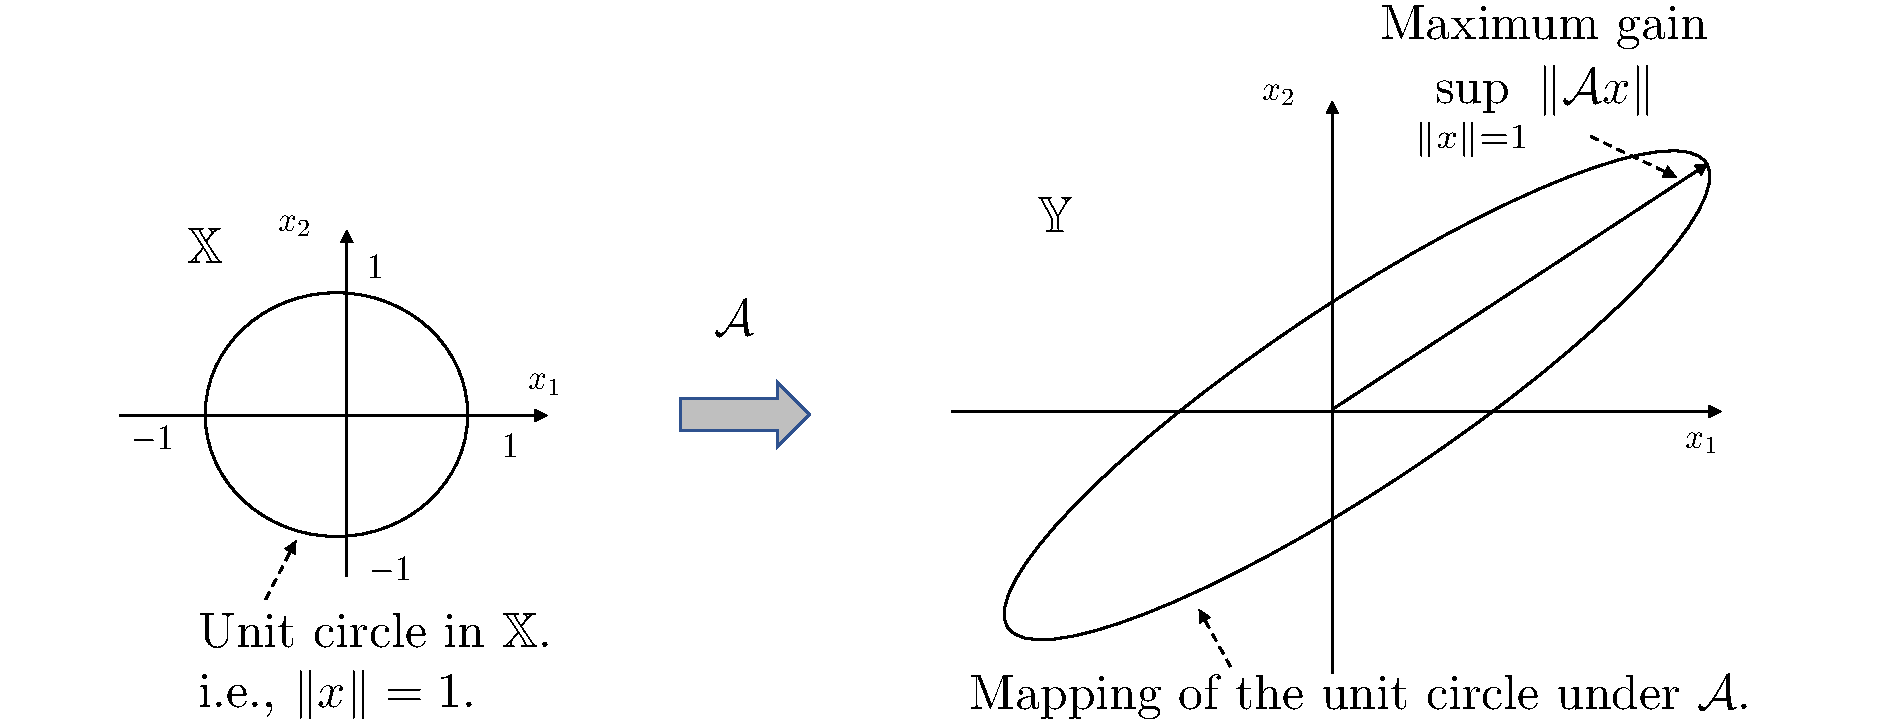
\includegraphics[width=4in]{figures/chap4_matrix_norm}	
	\end{center}
\end{frame}

%----------------------------------
\begin{frame}\frametitle{Norm of a Linear Operator, System Interpretation}
	Given a linear system
	\begin{center}
		
\includegraphics[width=2in]{figures/chap4_linear_system}	
	\end{center}

	\vfill
	
	The norm of the system $H(s)$ is the maximum gain of the system.
\end{frame}

%----------------------------------
\begin{frame}\frametitle{Norm of BIBO System}
	Let $\mathcal{A}: L_{\infty} \to L_{\infty}$ be an LTI system that is BIBO stable with impulse response $h(t)$, then
	\begin{align*}
	y(t) &= \int_0^t h(t-\tau)u(\tau)d\tau \\
		&\defeq \mathcal{A}[u] 
	\end{align*}
	
	\vfill
	
	Find $\norm{\mathcal{A}}_{\infty}$.
\end{frame}

%----------------------------------
\begin{frame}\frametitle{Norm of BIBO System, cont}
	\begin{lemma}
	\begin{align*}
	\norm{\mathcal{A}}_{\infty} &= \norm{h}_{L_1[0,\infty]} \\
		&\defeq \int_0^{\infty} |h(t)|dt 
	\end{align*}
	\end{lemma}
	
	\begin{proof}
		We need to prove two things
		\begin{enumerate}
		\item $\norm{\mathcal{A}}_{\infty} \leq \displaystyle\int_0^{\infty} |h(t)|dt$
		\item $\displaystyle\int_0^{\infty}|h(t)|dt \leq \norm{\mathcal{A}}_{\infty}$
		\end{enumerate}
	\end{proof}
\end{frame}

%----------------------------------
\begin{frame}\frametitle{Norm of BIBO System, Proof}
	\underline{Proof of 1.}

	\begin{align*}
		\sup_{\norm{x}_{\infty} = 1} \norm{\mathcal{A}[u]}_{\infty} &= \sup_{\norm{u}_{\infty} =
  		1} \norm{ \int_0^t h(t - \tau) u(\tau) d\tau  }_{\infty}
		\\
		&= \sup_{\norm{u}_{\infty} = 1} \left[ \sup_{t > 0} \abs{
  			\int_0^t h(t-\tau)u(\tau)d\tau} \right]\\
		&\leq \sup_{\norm{u}_{\infty} = 1} \left[ \sup_{t > 0}
  			\int_0^t \abs{ h(t-\tau)u(\tau)} d\tau \right]\\
		&\leq \sup_{\norm{u}_{\infty} = 1} \left[ \norm{ u }_{\infty} \sup_{t > 0} \int_0^t \abs{ h(t - \tau)} d\tau
			\right]\\
		&\leq \int_0^{\infty} \abs{h(\tau)}d\tau = \norm{h}_{L_1[0,\infty]}
	\end{align*}
\end{frame}

%----------------------------------
\begin{frame}\frametitle{Norm of BIBO System, Proof}
	\underline{Proof of 2.}
	
	Let $\hat{u}_t(\tau) = \begin{cases}
			1 & \text{ if } h(t-\tau) \geq 0\\
			-1 & \qquad \text{ otherwise }
			\end{cases}$.

	Note that $\norm{\hat{u}_t}_{\infty} = 1$ $\forall t>0$, we have that
	\[ 
		\int_0^t h(t-\tau)\hat{u}_t(\tau)d\tau = \int_0^t \abs{h(t - \tau)} d\tau.
	\]
	Therefore for this particular choice of $\hat{u}_t$ we have that
	\[ 
		\sup_{t > 0} \left[ \int_0^t \abs{h(t-\tau)}d\tau\right] = \norm{ A\hat{u}_\infty }_{\infty} = \int_0^{\infty} \abs{h(\tau)}d\tau.
	\]
	By definition of $\sup$
	\[ 
		\int_0^{\infty} \abs{h(\tau)}d\tau = \norm{ A\hat{u}_\infty }_{\infty} \leq
		\sup_{\norm{u}=1} \norm{Au}_{\infty}.
	\]
\end{frame}

%----------------------------------
\begin{frame}\frametitle{Operator Norm: Proof Technique}
	The proof technique shown here is the general approach to show that the norm of an operator is some value. 
	
	\vfill 

	Suppose that you would like to prove that
	\[ 
	\norm{\mathcal{A}} = M.
	\]
	You need to show two things
	\begin{enumerate}
		\item $\norm{\mathcal{A}} \leq M$
		\item $M \leq \norm{\mathcal{A}}$.
	\end{enumerate}
\end{frame}

%----------------------------------
\begin{frame}\frametitle{Operator Norm: Proof Technique}
	To show (1) use triangle and other inequalities to show that 
	\[ 
	\norm{\mathcal{A}x} \leq M\norm{x} 
	\]
	which implies that
	\[ 
	\sup_{\norm{x} = 1} \norm{\mathcal{A}x} \leq
		\sup_{\norm{x}=1} M\norm{x} = M 
	\]

	\vfill
	
	To show (2), construct a specific $\hat{x}$ such that
	\[ 
	\norm{ \hat{x} } = 1 \text{ and } \norm{ \mathcal{A}\hat{x} } = M.
	\]
	This implies that
	\[ 
		M \leq \sup_{\norm{x}=1} \norm{\mathcal{A}x} = \norm{\mathcal{A}}.
		\]	
\end{frame}

%----------------------------------
\begin{frame}\frametitle{Properties of Linear Operators}
	\begin{lemma}
		For any induced operator norm,
		\[ 
		\norm{\mathcal{A}x} \leq \norm{\mathcal{A}}\norm{x}. 
		\]
	\end{lemma}
	
	\begin{proof}
		\[ 
		\norm{\mathcal{A}} = \sup_{x \neq 0} \frac{\norm{\mathcal{A}x}}{\norm{x}}.
		\]
	Therefore for any $x \neq 0$ we must have that
	\begin{align*}
	&\norm{\mathcal{A}} \geq \frac{\norm{\mathcal{A}x}}{\norm{x}} \\
	\Rightarrow & \norm{\Acal x} \leq \norm{\mathcal{A}}\norm{x}.
	\end{align*}
	\end{proof}	
\end{frame}

%----------------------------------
\begin{frame}\frametitle{Properties of Linear Operators, cont}
	\begin{lemma}
		All induced operator norms satisfy the ``submultiplicative property,'' i.e.,
		\[ 
			\norm{\mathcal{A}\mathcal{B}} \leq \norm{\mathcal{A}}\norm{\mathcal{B}} 
			\]
	\end{lemma}
	
	\begin{proof}
		\begin{align*}
		\norm{\mathcal{A}\mathcal{B}} &= \sup_{\norm{x}=1}\norm{\mathcal{A}\mathcal{B}x} \\
				  &\leq \sup_{\norm{x} = 1} \norm{\mathcal{A}}\norm{\mathcal{B}x} \\
				  &\leq \sup_{\norm{x}=1}\norm{\mathcal{A}}\norm{\mathcal{B}}\norm{x} \\
				  &= \norm{\mathcal{A}}\norm{\mathcal{B}}
		\end{align*}
	\end{proof}
\end{frame}

%----------------------------------
\begin{frame}\frametitle{Properties of Linear Operators, cont}
	\begin{definition}
		An operator $\mathcal{A}:\mathbb{X}\to \mathbb{Y}$ is \underline{bounded} if
		$\norm{\Acal} < \infty$
	\end{definition}
	
	\vfill

	\begin{definition}
		The following three statements are equivalent
		\begin{enumerate}
			\item $\Acal:\mathbb{X}\to\mathbb{Y}$ is \underline{continuous}
			\item $x_n \to x^\ast \Rightarrow \Acal[x_n] \to \Acal[x^\ast] $ for all convergent sequences in $\mathbb{X}$
			\item $\forall \epsilon > 0, \quad \exists \delta > 0$ such that
				\[
				\norm{x - y} \leq \delta \quad \Rightarrow \quad \norm{ \Acal[x]-\Acal[y] } < \epsilon \qquad \forall x,y \in \mathbb{X} 
				\]
		\end{enumerate}
	\end{definition}
\end{frame}

%----------------------------------
\begin{frame}\frametitle{Properties of Linear Operators, cont}
	\begin{theorem}[Moon Theorem 4.1]
		A linear operator is bounded iff it is continuous.
	\end{theorem}

	\begin{proof}\end{proof}
	($\Rightarrow$) Suppose $\norm{ \Acal }=M < \infty$,let $\{x_n\}$ be any convergent sequence with limit $x^\ast\in\mathbb{X}$, then 
	\begin{align*}
	\norm{ \Acal x_n - \Acal x^\ast } &= \norm{ \Acal(x_n-x^\ast) } \leq \norm{ \Acal }\norm{x_n-x^\ast }\\
		&= M\norm{ x_n-x^\ast }\to 0 \Rightarrow \norm{\Acal x_n-\Acal x^\ast }\to 0.
	\end{align*}
	Therefore $\Acal$ is continuous.
	
\end{frame}

%----------------------------------
\begin{frame}\frametitle{Proof, cont}
	\noindent ($\Leftarrow$) Assume $\Acal$ is continuous and let $\epsilon = 1$ and $y = 0$ then $\exists \delta$ such that $\norm{ x } \leq \delta \Rightarrow \norm{ \Acal x } < 1$
	
	\vfill 

	Now let $0 \neq x \in \mathbb{X}$ be arbitrary, then 
	\[ 
	\norm{ \frac{\delta x}{\norm{ x }} } = \frac{\delta}{\norm{x}}\norm{ x } = \delta \leq \delta 
	\]
	implies that
	\[
		\norm{\Acal\left( \frac{\delta x}{\norm{ x }}\right)} = \frac{\delta}{\norm{ x }}\norm{ \Acal x } < 1
	\]
	which implies that
	\[
	\norm{ \Acal x } \leq \frac{1}{\delta}\norm{ x }
	\]
	
	\vfill
	
	Therefore $\Acal$ is bounded.
\end{frame}

%----------------------------------
\begin{frame}\frametitle{Properties of Linear Operators, cont}
	\begin{theorem}[Moon Theorem 4.2]
		Let $\Acal:\mathbb{X}\to\mathbb{Y}$ be a linear operator.  If $\mathbb{X}$ is a finite dimensional Hilbert space, then $\Acal$ is bounded.
	\end{theorem}
	
	\begin{proof}\end{proof}
		Let $\dim(\mathbb{X}) = n$ and let $\{p_1, \cdots p_n\}$ be an orthonormal basis for $\mathbb{X}$, then
		\[ 
		x = \sum_{k = 1}^n \iprod{ x,p_k} p_k
		\]
\end{frame}

%----------------------------------
\begin{frame}\frametitle{Proof, cont.}

	Define $D = \max\{ \norm{ \Acal p_1 }, \norm{\Acal p_2 }, \ldots, \norm{\Acal p_n}\}$ then
	\begin{align*}
		\norm{\Acal x} &= \norm{\Acal\left( \sum_{k=1}^n \iprod{ x,p_k} p_k\right) } \\
			&\leq \sum_{k=1}^n \abs{\iprod{ x,p_k}}\norm{\Acal p_k } \\
			&\leq D\sum_{k=1}^n \abs{\iprod{ x,p_k} } \\
			&\leq D \sum_{k=1}^n \norm{ x }\norm{ p_k } \qquad{(Caucy-Schwartz)}\\
			&= D n \norm{ x }  \\
	\end{align*}
	
	Therefore $\Acal$ is bounded.	
\end{frame}



\end{document}